% Original Paper can be found at http://hdl.handle.net/20.500.12648/1782 %

\documentclass[titlepage, 12pt]{article}
\usepackage{xcolor}
\usepackage[margin=1in]{geometry}
\usepackage{graphicx}
\usepackage{subcaption}
\usepackage{parskip}
\usepackage{natbib}
\usepackage{url}
\usepackage{titling}
\usepackage{sectsty}

\allsectionsfont{\centering}
\setcounter{secnumdepth}{0}

\begin{document}

	\begin{titlingpage}
	\centering
    	{\huge\bfseries Evaluating Cloud-Based Gaming Solutions\par}
    	\vspace{2cm}

	{\Large  A Master’s Thesis Project \\}	
	{\Large  Presented to the \\}	
    	{\scshape\LARGE Department of Communications and Humanities \par}
	
	\vfill
    	{\Large  In Partial Fulfillment \\}	
	{\Large  of the Requirements for the \\}
    	{\scshape\LARGE Master of Science Degree \par}
	
	\vfill
	{\LARGE State University of New York \par}
	{\LARGE Polytechnic Institute \par}

	\vfill
	{\Large By Daniel Truong\par}
	{\large May 2021\par}
	\end{titlingpage}

\section{Abstract}

Recently, tech companies such as Google and Microsoft have invested resources into offering cloud-based delivery of video games. Delivery of games over such a medium negates the need of requiring dedicated video game consoles or computers with robust 3D graphics hardware. Tangible hardware requirements for traditional video game playing are currently undergoing a supply shortage due to a multitude of factors, particularly related to the COVID-19 pandemic.

This project evaluates the cost of using cloud services vs. using a physical video game console. Also, this article evaluates whether players can come up with a custom solution utilizing VPS (virtual private server) providers such as Amazon Web Services. By utilizing the diffusion of innovations theory, we evaluate how the common actors of the video game industry try to replicate the traditional video game playing experience, but in a cloud setting. Results confirm that those wishing to use cloud-based services should only need a consumer-level personal computing device (such as a laptop or smartphone) to access them. Consumers must also take heed of their networking infrastructure, as well as the supported library of games that each service carries if they intend to maximize their value for each cloud service.

\newpage

\tableofcontents

\newpage

\section{Introduction}

In the mid-1990s, developers started developing games that took advantage of three-dimensional (3D) space and modeling. Rendering models in 3D was computationally expensive and often not smooth to animate. One of the earlier attempts at introducing 3D models to video games, Star Fox, required a special separate chip (the Super FX chip) to mathematically compute the rendering of 3D polygons on the screen.

Enter 3D accelerator cards. These cards were created to offload the computational labor of rendering 3D models to a processing unit separate from the main CPU: the Graphics Processing Unit (GPU). Companies such as 3dfx and Nvidia developed these add-on cards to complement contemporary 3D games such as Quake, Tomb Raider, and Resident Evil. Today, it is almost entirely necessary to possess a GPU in a modern personal computer or video game console to render 3D graphics effectively. Modern video game consoles contain proprietary GPUs that are dedicated to rendering the highly detailed 3D graphics that modern games sport today. As such, video game hardware is closely resembling that of PC gaming hardware (particularly in the shared x86-64 CPU instruction set). The line that separates video game consoles from personal computers (capable of playing video games) is becoming blurrier to distinguish (even as more console-exclusive games like Death Stranding and Days Gone are being released for the PC platform).

Since the beginning of the COVID-19 pandemic, GPUs and video game consoles have become incredibly difficult for ordinary consumers to acquire due to a lack of supply. Factors affecting supply include an increase in market demand due to players staying home and requiring video game hardware, scalpers taking advantage of "FOMO" (fear of missing out) by purchasing hardware en masse in hopes of reselling above MSRP, cryptocurrency mining operations, and a shortage in semiconductor material necessary for the manufacture of GPUs.

In 2019, Google and Microsoft debuted cloud-based gaming services that were powered by their own data centers. Google Stadia and Microsoft’s Xbox Cloud Gaming (previously known as Project xCloud) allow gamers to play video games over the internet without requiring a dedicated video gaming console. Gamers could play games from an inexpensive, lower-spec computer or a tablet. The only costs that the gamers would need to handle are either subscription-based or licensing fees for individual video games.

\section{Literature Review}

Microsoft and Google are not the first companies to attempt the endeavor of cloud gaming. In 2005, a company called OnLive was formed. How OnLive worked was that users could "rent" video games and play them without installing them onto a computer (or requiring physical media to order). At the time of its release, there were growing concerns that OnLive's networking required more robust bandwidth and mitigated latency to perform properly \citep{multimedia-systems3}. Around that time, a study on potentially utilizing edge servers to optimize gaming performance found that the infrastructure of that time was insufficient for cloud gaming needs \citep{multimedia-systems2}.

In addition, Microsoft took umbrage with how OnLive was leveraging the Windows 7 operating system to provide virtual environments for the games to run in \citep{macworld}. OnLive would eventually shut down in 2012 and be bought up by Sony Computer Entertainment in 2015. This would not be the first company Sony bought that dealt with cloud gaming; in 2012, Sony bought the game streaming company Gaikai for \$380 million \citep{engadget}. Gaikai was initially formed to be the “Netflix” of gaming, in the sense of being able to browse a catalog of games and being able to play them over the cloud. Sony would eventually incorporate tech from both companies to power its PlayStation Now service.

\section{Current State of the Video Game Industry}

Since 2001, companies like Sony, Microsoft and Nintendo have long established themselves as institutions within the video game industry. As such, their roles in the video game industry have allowed them to steer the direction of innovation with each new successive console generation. Based on a study done by Thomas Backer and Everett Rogers in 1998, there exists this notion called a “diffusion of innovations” that posits that a new idea is gradually adopted, then rapidly implemented if that new idea is successful. Applying diffusion of innovation theory to the video game industry, we have one such example with Microsoft: since Microsoft also specializes in consumer desktop operating systems (Windows), we see that they have also used the same codebase for the Xbox One. This has made it easier for developers to create PC versions of the same game that they would have created for the Xbox One. And because of how streamlined the process became, the same principle was applied to the Xbox Series X|S. The same idea would also be implemented by Sony for their Playstation 4 and 5 consoles. 

Right now, because Sony, Microsoft and Nintendo dominate the video game industry, they are able to influence the innovation of video gaming technology; particularly cloud gaming. Actors such as Google and Nvidia are relatively new to the video game platform market, yet were some of the first (since OnLive and Gaikai) to have a cloud gaming service implemented. Since then, Sony and Microsoft have also come out with their own cloud gaming services. Via diffusion of innovation, adoption of cloud gaming services by users are going to be largely driven by them should the supply of game consoles and GPUs not improve over time.

Typically, this is how cloud gaming is implemented: The Client has a display, a video decoder, and a game control device (controller). The Cloud contains the game engine and a video encoder. The Client feeds input data to their controller; this data gets sent over IP to the game engine in the cloud. The game engine then feeds visual stimulus data to the video encoder. The video encoder sends that data back to the client via the video decoder. The decoder then produces graphical elements to give to the display \citep{multimedia-systems}.

One of the biggest pitfalls that prevent an enjoyable experience for cloud gaming is latency. PCWorld defines latency as "the time it takes…to input a controller movement…and for the game to respond accordingly" \citep{pcworld}. To combat issues like latency, region-based hosting was looked at as a viable solution \citep{conf}. Future development in determining hosting regions is slated to heavily involve AWS, which contains high-performing compute instances that can be scaled by region.

In addition to using AWS, several other technologies could come into play to benefit cloud gaming. With 5G cellular signals being gradually rolled out, this could allow mobile phone users to play cloud-based games in an ideal manner. The newest standard for wireless local area networks (802.11ax, aka Wi-Fi 6) seeks to improve performance by implementing orthogonal frequency division multiple access (OFDMA) and multi-user multiple input multiple output (MU-MIMO) to achieve a max speed of 9.6 Gbps \citep{mobile-networks}.

Video streaming services such as Netflix and Hulu have established their business model to allow users to select videos to watch immediately without requiring individual downloads. With how services like Xbox Cloud Gaming and Stadia are structured, users don’t need to download games and can play them right away. Parallels can be drawn between video entertainment services and cloud gaming services when it comes to ideas on how to best implement cost and pricing schedules.

\section{Externalities Affecting Cloud Gaming}

One of the downsides of cloud gaming is the high networking speed requirements. Users must be subscribed to (at least) a 25 Mbps network connection with minimal latency to utilize all the cloud gaming services to their fullest feature set. According to the 2020 Broadband Deployment Report from the FCC: in 2018, 94.4\% of the US population was reported to have access to high-speed internet. The report acknowledges that while this is net increase from 2017’s figure (93.5\%), there still exists a sizeable population size that lack access to high-speed internet. In addition, this division in access can be attributed to pre-dominantly rural areas; 22.3\% of Americans in rural areas lack high-speed internet, compared to 1.5\% in urban areas lacking high-speed internet. Bridging this divide between rural and urban users is going to require investment in networking infrastructure amongst rural areas; particularly this infrastructure must facilitate low latency for cloud gaming services to operate with minimal flaws. 

While users aren't required to have the latest GPU in their computer to play cloud-gaming services, they must have a computer that is (at the very least) capable of high-definition video processing (i.e. newer Intel integrated GPUs) to mitigate input lag and deliver optimal gameplay quality. This isn't to say that users must go out and purchase newer computing equipment to play cloud-based games; rather consumer education is required to ensure that either their current hardware is capable of playing these games or if slightly more robust hardware is required.

\section{Project Purpose}

With the lack of supply for video game consoles and PC gaming hardware, the purpose of this project is to evaluate if simply having a computer or phone and a cloud gaming subscription is a sufficient alternative. In addition, with cloud computing platforms such as Amazon Web Services or Google Cloud Platform, can they serve as a viable alternative to owning a gaming computer? For this project, while console gaming and PC gaming are distinct from each other, both will be treated as the same (much like how PC gaming was an alternative to video game console ownership in the past).

Part of the review process will evaluate the costs of the video game consoles and gaming PCs compared with the cloud subscription services. When it comes to owning a game console like the Xbox Series X|S or the PlayStation 5, consumers will also need to consider their accompanying online subscription services to make the most out of their consoles (particularly if players intend to play multiplayer games online). The previous two game console generations (7th gen: Xbox 360, Playstation 3, Nintendo Wii; 8th gen: Xbox One, Playstation 4, Wii U, Switch) lasted approximately 7 years before the next generation was introduced. As such, the cost of subscribing to cloud gaming services will be calculated over a 7-year term.

\section{Testing Methodology}

Five cloud-based solutions were evaluated: Google Stadia, Xbox Cloud Gaming, PlayStation Now (PS Now), Nvidia's GeForce Now, and a custom solution involving virtual private servers (VPS) hosted on Amazon Web Services (AWS).

	\subsection{Google Stadia}
	
	No subscription is required to play games. Games are buy-once, play forever. A subscription (Stadia Pro) costs \$9.99 per month and allows access to specific free games. An internet connection speed of at least 10 Mbps is required to use Stadia; 35 Mbps is recommended at a minimum to stream games in 4K resolution.
	
	\subsection{Xbox Cloud Gaming}
	
	Requires a subscription to Game Pass Ultimate (\$14.99 per month) and ownership of Xbox Wireless Controller (MSRP \$59.99). Comes with access to free games curated by Microsoft. An internet connection speed of at least 7-10 Mbps is required.
	
	\subsection{PS Now}
	
	Requires a monthly subscription fee (\$9.99 per month) and ownership of a DualShock 4 controller (MSRP \$59.99). Offers access to free games curated by Sony; games range from the PlayStation 2 to PlayStation 4 era. An internet connection speed of at least 5 Mbps is required.
	
	\subsection{GeForce Now}
	
	No subscription is required to play games. However, the free tier is limited to session lengths of one hour and subject to peak access wait times. Priority subscription costs \$9.99 per month and removes these limitations. Games are bought once on supported marketplace platforms (Steam, GOG.com, Epic Games Store). GeForce Now requires 15 Mbps internet speeds for 720p streaming or 25 Mbps for 1080p.

	\subsection{Custom VPS Solution}
	
	To adequately replicate a gaming PC, a "g4dn.xlarge" virtual machine instance will be generated on AWS's Elastic Compute Cloud (EC2) platform. This virtual instance comes with 4 virtual CPU cores, 16 GBs RAM, a 125 GB NVMe SSD storage partition, an Nvidia T4 GPU and runs Windows Server 2019 as its OS (functionally replicating Windows 10 v1809). Operation of the g4dn.xlarge instance will cost \$0.71 per hour and \$0.10 per GB storage on a monthly basis.
	
	Whereas the virtual machines are running Windows 10 in a cloud environment, normally the Microsoft Remote Desktop client or any RDP (Remote Desktop Protocol) compliant client would be used to interface with the servers. However, RDP is not designed to render GPU-accelerated data over IP. As such, to connect to the VM on EC2, Parsec will be used to provide video feed encoding for both the client and the gaming VM. Parsec is free for personal usage but comes with a premium tier for \$9.99 per month that allows for privacy mode, dual monitor streaming, and a 4:4:4 color mode. There is also an enterprise plan for \$35 per user/month that adds SAML authentication and VIP support. Information on setting up the custom VPS solution can be located under Appendix A.
	
	To test connecting to the cloud-gaming services, a client computing system was needed. This client will replicate an average consumer laptop that is not capable of playing games on native hardware. In 2020, Gartner Research recommended the following configurations for a “Traditionally Mainstream” Windows 10-based desktop and laptop:

	\begin{itemize}
	\item {CPU (Desktop): Intel Core i5-10500 or AMD Ryzen 5 Pro 3600}
	\item {CPU (Laptop): Intel Core i5-10310U or AMD Ryzen 5 Pro 3500U or 4650U}
	\item {Memory: 16 GBs DDR3}
	\item {Hard Drive: 256 GB Solid State Drive}
	\item {GPU (Graphics Processing Unit): Integrated}
	\end{itemize}

	It must be noted that Gartner Research’s recommendations are typically oriented towards enterprise use-case; in particular, the aforementioned specs are geared towards users “offering adequate performance and capabilities to support most workplaces activities” \citep{gartner}. Since consumer PCs and laptops are being built with stronger and newer configurations \citep{pcworld2}, Gartner’s specifications will be perfect as a baseline to test cloud gaming services against.
	
	To replicate a consumer PC for testing, a laptop will be configured with the following specs:
	
	\begin{itemize}
	\item {CPU: Intel Core i5-7360U}
	\item {Memory: 16 GB LPDDR3}
	\item {Hard Drive: 256 GB SSD}
	\item {GPU: Intel Iris Plus Graphics 640 (integrated)}
	\item {Operating System: Windows 10 64-bit (Build 19042.906)}
	\item {Wi-Fi Card: Broadcom 802.11ac Network Adapter}
	\end{itemize}
	
	At the time of writing (April 4th, 2021), Xbox Cloud Gaming currently does not have a client for Windows-based PCs; it is only available for Android-based smartphones. As such, an Android smartphone (with the following specs) will be used for testing purposes of Xbox Cloud Gaming.
	
	\begin{itemize}
	\item {CPU: Qualcomm Snapdragon 820}
	\item {Memory: 4 GB LPDDR4}
	\item {Storage: 32 GBs}
	\item {GPU: Adrena 530}
	\item {Operating System: Android 8.0.0}
	\end{itemize}
	
	With regards to networking infrastructure, the test environment will operate on a 5 GHz, 802.11ac wireless network. Speeds are configured at 200/10 Mbps download/upload (respectively). Network latency was recorded at 26 ms at the time of the initial setup.
	
	The review process for all services (including the custom VPS solution) will consider the following variables:
	
	\begin{itemize}
	\item {Visual glitches and bugs}
	\item {Input latency}
	\item {Game library support}
	\end{itemize}
	
	The cost of the services, compared to the physical contemporary equivalent hardware and associated costs, will be utilized towards determining if whether cloud gaming is a viable alternative to owning a video game console or gaming computer.

	\subsection{Games Tested}
	
	Due to platform licensing restrictions, the same games could not be evaluated across all the services. In any case, the games selected represent varying genres: first-person shooters (FPS), fighting, racing, turn-based strategy, and role-playing games. Some of these games have a synchronous multiplayer component which will be reviewed during testing.
	
	\begin{itemize}
	\item {Hitman (Google Stadia): a single-player stealth action game.}
	\item {Republique (Google Stadia): single-player action-adventure game.}
	\item {Superhot: Mind Control Delete (Google Stadia): single-player first-person action game.}
	\item {F1 2020 (Google Stadia): single/multiplayer racing game.}
	\item {Gears 5 (Xbox Cloud Gaming): single/multiplayer action game with team-based and competitive elements.}
	\item {Doom Eternal (Xbox Cloud Gaming): single-player FPS action game.}
	\item {Forza Horizon 4 (Xbox Cloud Gaming): single/multiplayer racing game.}
	\item {Octopath Traveller (Xbox Cloud Gaming): single-player role-playing game.}
	\item {Street Fighter V (PS Now): single/multiplayer competitive fighting game.}
	\item {Horizon Zero Dawn (PS Now): single-player adventure game.}
	\item {Rage 2 (PS Now): single-player FPS action game.}
	\item {MX vs. ATV All Out (PS Now): single/multiplayer racing game.}
	\item {Rainbow Six Siege (GeForce Now): multiplayer FPS team-based competition game.}
	\item {South Park: The Stick of Truth (GeForce Now): single-player turn-based role-playing game.}
	\item {Just Cause 3 (GeForce Now): single-player action-adventure game.}
	\item {Team Fortress 2 (GeForce Now): multiplayer FPS team-based game.}
	\item {Counter-Strike: Global Offensive (Custom VPS Solution): multiplayer FPS competitive team-based shooter.}
	\item {Crysis (Custom VPS Solution): single-player FPS action game.}
	\item {Cyberpunk 2077 (Custom VPS Solution): single-player FPS action game.}
	\item {XCOM 2 (Custom VPS Solution): single-player turn-based strategy game.}
	\end{itemize}

\section{Outcomes}

For the most part, all services performed relatively well from a technical standpoint. Stadia and GeForce Now ran smoothly at higher resolutions; a steady 60 FPS frame rate was maintained at a resolution of 1920x1080. PS Now had some graphical artifacts that appeared during gameplay, as well as intermittent stuttering. All services, save for Xbox Cloud Gaming, experienced mild input lag. Xbox Cloud Gaming was limited to testing on Android smartphones and had a noticeable input lag that adversely affected gameplay performance in games like Gears 5 and Doom Eternal.

One thing that must be noted: the emulated hardware for Xbox Cloud Gaming and PlayStation Now is based on 8th generation video game consoles (Xbox One S and PlayStation 4 respectively). This is done to maintain maximum compatibility with the available library of games for each service. Upgrades to the 9th generation of consoles are reportedly in development at the time of writing \citep{vg247}.

Game availability for all platforms was widely varied. Stadia Pro only had 26 games available to try for free; other games had to be purchased individually. GeForce Now relies on select supported games that were pre-bought on Steam, GOG, or Epic Games Store - over 2000 games are supported. Xbox Cloud Gaming and PS Now tap into a wide gaming library that includes the current-gen and the prior 2 generations of games. This library however dynamically changes (based on license availability) and can be concurrently accessed via their respective platform's subscription plan.

	\subsection{Custom VPS Solution}
	
	The custom VPS solution performed just as well as Google Stadia and GeForce Now, save for minor artifacting and input lag (possibly due to how Parsec handles video compression). Because the custom VPS solution emulated the effect of having a gaming PC, the game library was dependent on services such as Steam, GOG, Epic Games Store, uPlay, etc. The setup of the gaming VM came with moderate difficulty; once the VM was generated, special video and audio drivers from Nvidia and Razer (respectively) needed to be installed to have the VM function properly. Also, special commands were necessary to disable the "Microsoft Basic Display Adapter" for Parsec to function properly. Finally, configuration was needed on EC2 to keep the IP address static and the storage persistent to prevent requiring reinstallation of games and requisite applications.

\section{Cost Analysis}

When it comes to using cloud gaming services over traditional consoles, costs appeared higher at first glance. Each service (that included games in its library) calculated over a 7-year time frame came out to between \$839.16 and \$1319.15. Comparing that to the initial cost of the Playstation 5 and Xbox Series X high-end models (\$499.99), it would appear that the cloud services were more expensive over the standard 7-year generational lifetime. However, the cost of the consoles does not consider monthly subscription fees (mandatory for playing online multiplayer games). The cloud-based services have multiplayer fees built into their subscription model, as well as a library of curated games that are available for the player to access.

Considering the leftover costs from each cloud service (after being subtracted from their respective console’s MSRP), if one were to purchase brand new games from those leftover costs (at the standard AAA price rate of \$59.99 per game), each service would at least need to offer at most 13 games concurrently to match their physical counterpart's value. As it stands, except for GeForce Now, all the other services offer up readily accessible games that exceed the value of owning a physical console (see Appendix B for the complete figures on each service and their costs).

As for supplanting PC gaming (particularly with GeForce Now or the custom VPS solution), this is where costs become somewhat complicated. Yearly, GeForce Now costs \$119.88. It offers up access to a virtual computing environment to play PC games with, but those games must be purchased separately and supported by the platform (dependent on publisher license authorization). As for the custom VPS solution, because server resources are charged by the hour (when active), a holistic approach must be taken towards analyzing monthly or yearly usage. A policy statement by the American Academy of Pediatrics recommended that total entertainment screen time be limited to 1-2 hours per day - particularly for young children \citep{pediatrics}. Assuming daily usage of 2 hours, that puts the monthly operational costs (including hourly server usage and monthly SSD storage) at \$56.52.

\section{Conclusion}

As it stands, cloud gaming shows quite a bit of promise with regard to supplanting physical console hardware for video gaming access. Provided an adequate client computing device and robust networking infrastructure, one could play the latest video games without requiring newer and pricier computing hardware or consoles. Externalities such as network latency or outages can affect the gameplay experience. In addition, depending on the service, available games are either curated from a pre-defined collection of authorized titles to play (Xbox Cloud Gaming, Playstation Now) or must be purchased outright on their respective platforms (Stadia, GeForce Now). Finally, until Sony and Microsoft upgrade the back-end hardware that is used for emulating their titles, players will be stuck with playing the 8th-gen version of games (which currently offer no higher than 1080p resolution for their games).

As it stands, there are a couple of threats that could affect player experience and any future development of cloud gaming. To reiterate on an early point, one of them is availability of high-speed internet. While this problem isn’t as exacerbated in urban locales, rural users may face certain difficulty with accessing cloud gaming services. Further development of networking infrastructure in rural areas is imperative for users should they choose to subscribe to cloud gaming services. Another threat users may face for cloud gaming are ISP data caps. Certain ISPs have a monthly limit on how much data a consumer can download at any given time. Having such a limit may affect advances in cloud gaming access (especially if higher resolution video streams such as 4K or 1440p are to be implemented). Either legislation to eliminate data caps will be necessary to eliminate this problem or cloud gaming services will need to work on optimizing their video streams for data transmission relative to the average market cap on data downloads
	
	\subsection{Future Business Forecast}
	
	As of April 4th, 2021, industry analysts were forecasting doubts about the long-term stability of Google Stadia. In February of 2021, Google shut down its internal gaming studio that would have made original titles for the Stadia platform \citep{techcrunch}. As it stands, Google must rely on third-party licensing rights to allow players to stream games from the Stadia platform. Meanwhile, Amazon announced that they were going to be joining the cloud gaming market with their new service called Luna. Amazon Luna is still currently in development at the time of writing and no indication has been given on its full release date. Finally. Nintendo is currently experimenting with delivering cloud gaming by allowing users to purchase access to select games and play them virtually with a Nintendo Switch. At the time of writing, only four games are available for cloud streaming (2 are exclusive to Japan).
	
	It remains to be seen how the future of cloud gaming will come into shape (and whether it will be an actual viable way to play video games many years forward). With the semiconductor shortage expected to last for at least another year \citep{verge}, we may see companies shift development on optimizing stimuli data to completely (or very nearly) replicate having a physical console. Furthermore, we may see a shift in licensing paradigm much in the way of how Spotify and Netflix changed the concept of digital media licensing from perpetual to subscription-based. Rather than outright owning the game, users might be facing a revolving door of differing games subject to publisher licensing rights towards the cloud gaming provider.

\newpage
\bibliographystyle{apalike}
\bibliography{apa-references}

\newpage
\section{Appendix A: How to Setup AWS for Cloud Gaming}

	\subsection*{Create EC2 Instance}

	Under the EC2 Dashboard, select \textbf{Launch Instance}. Configure the instance with the following options:

	\begin{enumerate}
	\item{Amazon Machine Image (AMI): \underline{Microsoft Windows Server 2019 Base}}
	\item{Instance Type: \underline{g4dn.xlarge}}
	\item{Instance Details: leave all settings as Default}
	\item{Add Storage: set \underline{size to 150 GB} and \underline{volume type to gp2}}
	\item{Add Tags: Optional (recommended if more than one server will be setup)}
	\item{Security Group:}
		\begin{enumerate}
		\item{Assign a security group: set to \underline{Create a new security group}}
		\item{Security group name: \underline{aws-gaming-pc} or something descriptive}
		\item{Description: Optional}
		\item{Add the following port rules:}
			\begin{enumerate}
			\item{TCP 3389 from Anywhere (RDP port)}
			\item{UDP 8000-12200 from Anywhere (Parsec port range)}
			\end{enumerate}
		\end{enumerate}
	\item{Review Instance Launch: confirm that your settings appear correct. Once ready, click Launch.}
	\item{Select an existing key pair or create a new key pair: create a new key pair and give it a descriptive name (i.e. aws-gaming-pc). Download the key pair and keep the file in a safe and secure location.}
	\end{enumerate}

	Once the EC2 instance is created, assign an elastic IP address to it for easier access.

	\begin{enumerate}
	\item{On the left-side menu, locate the \underline{Elastic IPs} option.}
	\item{Click the orange \underline{Allocate Elastic IP address} button.}
	\item{Under \underline{Elastic IP address settings}, select \underline{Amazon’s pool of IPv4 addresses}. Click \underline{Allocate}.}
	\item{On the \underline{Elastic IPs} section, check the box next to the newly associated IP address and go to \underline{Actions} - \underline{Associate Elastic IP address}.}
	\item{Associate Elastic IP address}
		\begin{enumerate}
		\item{Resource type: Instance}
		\item{Instance: select the EC2 instance created in the last section}
		\item{Private IP address: select the default IP that comes up}
		\item{Click \underline{Associate}.}
		\end{enumerate}
	\item{Go back to the \underline{Instances} section and refresh the page. Make note of the \underline{Public IPv4 address} as this will be used for connecting to the EC2 instance.}
	\end{enumerate}

	Before connecting to the EC2 instance, you will need an IAM (Identity \& Access Management) user to be able to download GPU drivers. 

	\begin{enumerate}
	\item{Go to \underline{console.aws.amazon.com/iam}}
	\item{Go to \underline{Users} - \underline{Add user}.}
	\item{Add user}
		\begin{enumerate}
		\item{User name: \underline{driver-dload}}
		\item{Access type: \underline{Programmatic access}}
		\end{enumerate}
	\item{Set Permissions}
		\begin{enumerate}
		\item{Attach existing policies directly}
		\item{Check \underline{Administrator Access}}
		\end{enumerate}
	\item{Tags: Optional}
	\item{Review the settings, then click \underline{Create user}.}
	\item{Copy the Access Key ID and Secret. Store these values in a safe and secure location.}
	\end{enumerate}

	\subsection*{Configure Cloud Gaming Server}

	Connect to the remote server (via Remote Desktop Connection) using the elastic IP address set in the previous steps

	\begin{enumerate}
	\item{On the EC2 \underline{Instances} section, check the box for your instance and click \underline{Connect}.}
	\item{Select the \underline{RDP client} tab.}
	\item{Click \underline{Download remote desktop file}.}
	\item{Click \underline{Get password} to get the logon password for the instance. Click Browse and select the key pair that was downloaded earlier. Then click Decrypt Password to get the logon password.}
	\item{Run the Remote Desktop file that was downloaded in Step 3. Login with the admin password gained from the last step.}
	\item{On the remote EC2 instance, change the Administrator password. }
		\begin{enumerate}
		\item{Press Windows key + R, then type in netplwiz.}
		\item{Click the \underline{Advanced} tab and select Advanced (under Advanced user management).}
		\item{Under the Users folder, right-click on Administrator and select Set Password.}
		\item{Set a new password. This will be used for Administrative functions, including logging in via RDP and Parsec.}
		\end{enumerate}
	\item{Open a Powershell prompt and run the below command. Follow the instructions and prompts that appear.}
		\begin{figure}[ht]
		\centering
		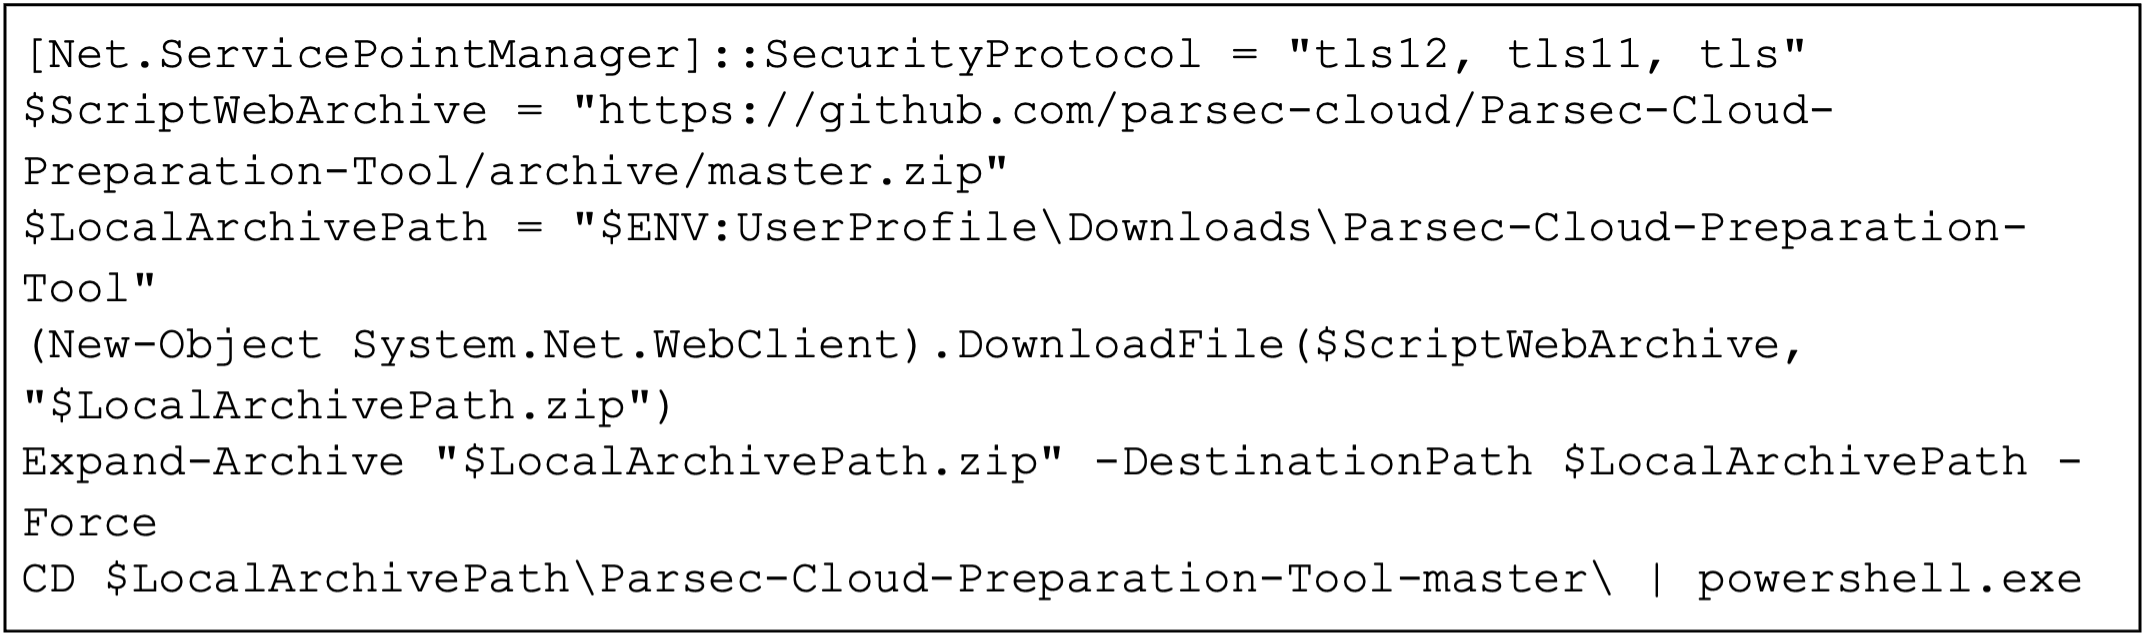
\includegraphics{powershell.png}
		\end{figure}
	\item{Once the installation process is complete, open Parsec and login.}
	\item{Go to Settings - Host and confirm that Hosting Enabled is set to Enabled.}
	\item{Go to Network and set the following Port options:}
		\begin{enumerate}
		\item{Client Port: \underline{12000}}
		\item{Host Start Port: \underline{12100}}
		\end{enumerate}
	\item{Disconnect from the Remote Desktop Session. On the client computer, install Parsec and login. You should then see the Cloud Gaming Server show up as an option to connect to. If you can access the desktop, then your Cloud Gaming Server is all set to use. }
	\end{enumerate}

	\subsection*{Recommended Cleanup Steps}

	\begin{itemize}
	\item {Adjust the port rule range for Parsec (under Security Groups) from \underline{UDP 8000-12200} to \underline{UDP 12000-12100}. }
	\item {Change the port rule for \underline{TCP 3389} (RDP) from Anywhere to your own IP address.}
	\item {Deactivate the \underline{driver-dload} IAM user if you do not anticipate updating the GPU drivers on a constant basis.}
	\item {Setup Auto-Shutdown (there is a script on the desktop to execute) so that the machine shuts down after idling for a while. This will be useful toward not incurring additional costs from idle usage.}
	\end{itemize}

\newpage
\section{Appendix B: Cloud Gaming Cost Data}

\begin{figure}[ht]
\centering
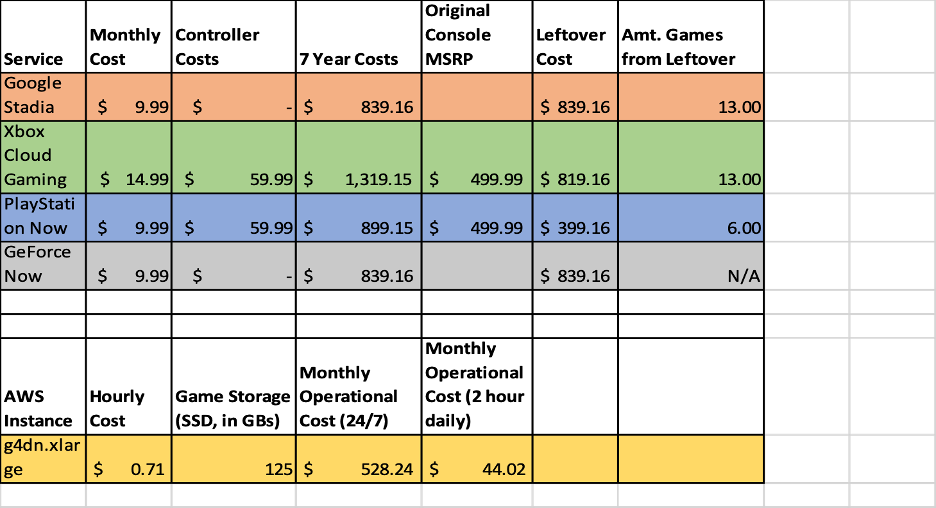
\includegraphics{costdata.png}
\end{figure}

\end{document}

